\chapter{Co-located Collaboration with Multi-user Immersive Display}
\label{chapter:colocated_colab}
\minitoc

\section{Introduction}
Immersive CVEs can be used to connect networked users to the same virtual place for collaboration. Users can be both geographically distributed or co-located at the same physical place. Compared to remote situations, co-located users share the same physical workspace which allows direct user communication and interaction without computer mediation, and unlike cases in which co-located users collaborate with 2D graphic user interface (e.g. image wall, interactive table), immersive CVEs allow them to share the same virtual world on top of the same real space.

A major problem of using immersive CVE for co-located collaboration is that classical projection-based immersive displays can only show images generated from a single user's viewpoint and others sharing the same images from another location will suffer visual distortion. To tackle this problem, multi-user immersive displays are designed to offer individual stereoscopic views for multiple users.

This chapter concentrates on how co-located users collaborate inside multi-user immersive virtual environment and it is divided into four sections. The first presents technical aspects related to multi-user immersive displays and summarizes existing methods to separate images for different users. The second describes notions that allow us to define two collaborative modes that form a general framework for co-located collaboration. Then the third section presents two major issues that we identify during the collaboration process and the last proposes research methodology that we adopted to solve the aforementioned issues.  


\section{Multi-user Immersive Display}
Immersive display constitutes a main component of immersive virtual environment as the visual sense plays a predominant role in user's perception process. As mentioned in previous chapter (section~\ref{sec:visual_interface}), immersive displays differ from traditional displays in that they have large field of view, high resolution, stereoscopic images associated with viewpoint tracking technology.


\subsection{Stereoscopy}
\label{sec:stereo}

Stereoscopy is the production of the illusion of depth by presenting a pair of 2D images showing two perspectives that both eyes naturally have in binocular vision. Then the brain merges the two images into a ``single" one to achieve stereopsis \citep{Blake2006Perception}. Besides stereoscopy, other cues (e.g. object occlusion, linear perspective, etc.) can also help to determine relative distances and depth in a perceived scene, but stereoscopy remains the most effective factor that provides users with instant depth perception.

To achieve stereoscopic vision, we should first generate a pair of images depending on user's head position and orientation, as well as the interpupillary distance (IPD) \citep{Dodgson2004IPD}. Then we need to provide two images separately for each eye. Existing separation methods can be classified into three categories:

\begin{itemize}
\item Head-mounted displays: we can put two small screens in front of the eyes, or a single screen displaying two images side by side to show only the desired image to each eye (Figure~\ref{fig:1_vi:hmd});
\item Auto-stereoscopic screen: auto-stereoscopic display separate images at the screen level by using the lenticular lenses or parallax barrier to assure that each eye of the user sees different pixel columns which correspond to two different images \citep{Perlin2000Autostereo};
\item Eyeglasses separation: images can be separated passively by colorimetric differentiation or polarized glasses, or actively by rapidly alternating shuttered glasses.
\end{itemize}

Each type of stereoscopic display has its advantages and inconveniences. HMD is the most straightforward way to provide two different images for the eyes and allows fully visual immersion of the user (the real world is completely blocked from user's eyes except for see-through HMDs \citep{Schmalstieg2002Stube}). However, various technical limitations like limited resolution and field of view enhance user's visual fatigue and restrain the wide use of HMDs. Unlike HMDs that are heavy to carry, eyeglasses based technology combined with large immersive projection display (e.g. image wall, CAVE, dome) gives user a more comfortable stereo experience. Auto-stereoscopic screens do not require user to equip any glasses or headgear, but have limited work range - user should stay at predefined position (at a certain distance from the screen) to correctly perceive stereo images.

Recent technical developments largely improved the usability of all three types of stereoscopic display. HMDs now are lighter and less expensive with more compact design, along with better resolution, larger field of view. The improvements of immersive projection technology (IPT) \citep{Bullinger1997Immersive} makes projection-based systems with eyeglasses a widespread solution both in academic institutes and industries, and they are specially useful to create large immersive virtual environment for group immersion by the combination of multiple projectors, such as CAVEs. Auto-stereoscopic screen combined with user tracking can now allow the tracked user to pass through different viewing areas without discontinuity \citep{Kooima2010Tiled}, but still requires complex hardware and software setup. So HMDs and projection-based systems become the major platform to support immersive or partially-immersive experience.


\subsection{Visual Distortion}
Stereoscopic images are generated from a single location - the center of projection (CoP) \citep{Banks2009Perception}. A user can properly perceive the displayed 3D content on a projection screen when viewed from the CoP. So in an immersive virtual environment, user's viewpoint is captured by head-tracking to serve as the CoP to generate appropriate images in real time as the user moves physically.

While HMDs provide personal stereoscopic images for a single user, projection-based systems are often shared by a group of people for team work, as shown by Figure~\ref{fig:2_group}. In such multi-user situation, only the tracked user receives correct stereo images from the CoP, other co-located users (followers) share the same stereo images intended for the tracked user and participate passively in the collaborative task \citep{Bayon2006Multiple}. When users are close enough to the tracked user, they can get a relatively faithful representation of the virtual environment, but as the distance increases, displacement from the CoP results in increasingly inappropriate stereo cues and distorted perception of the virtual space.

\begin{figure}[htb]
  \centering
  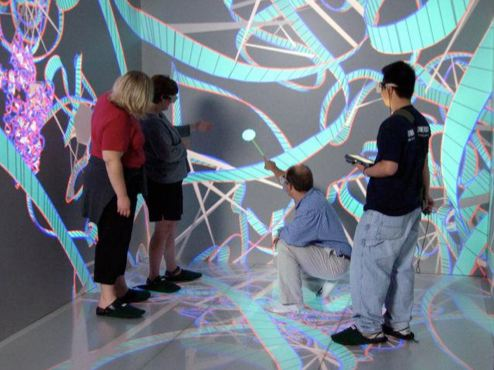
\includegraphics[width=0.6\textwidth]{figures/ch2/group}
  \caption{\label{fig:2_group}A group of people collaborating in a CAVE for data visualization \citep{Pollock2012Right}.}
\end{figure}

\begin{figure}[htb]
  \centering
  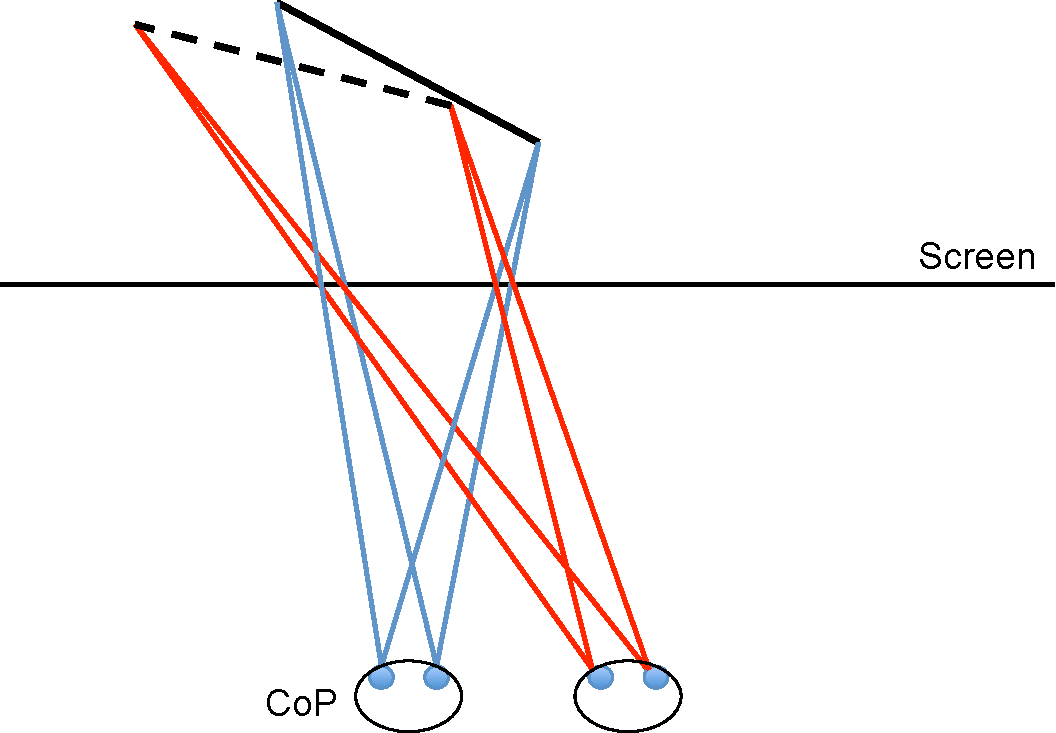
\includegraphics[width=0.48\textwidth]{figures/ch2/distortion_1}
  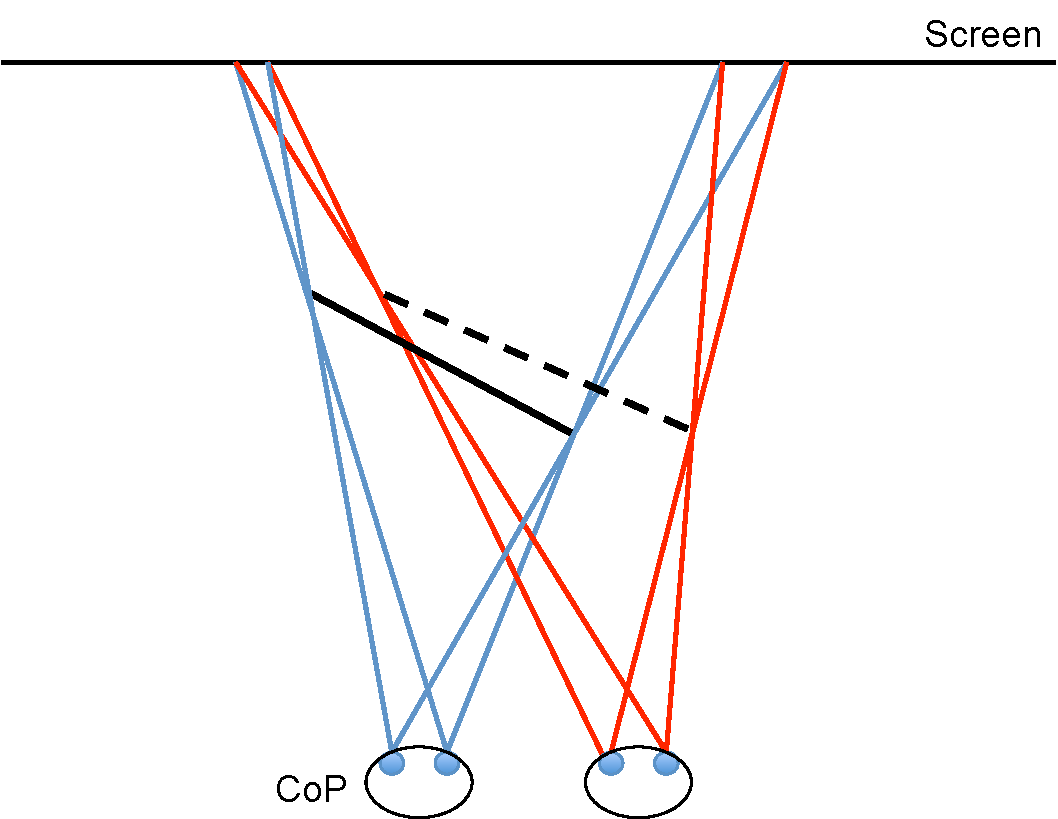
\includegraphics[width=0.48\textwidth]{figures/ch2/distortion_2}
  \caption{\label{fig:2_ray_model}Illustration of visual distortion by perceiving the right view from a location other than the CoP. The black line represents the correct view of object perceived from CoP and the dotted line corresponds the distorted view observed from another location.}
\end{figure}


Visual distortion caused by displacement from the CoP can be predicted by a ray-intersection model \citep{Burton2012Diagnosing}. As shown by Figure~\ref{fig:2_ray_model}, no matter the virtual object is situated behind or in front of the screen, a lateral displacement from the CoP will cause deformation and shift of the perceived object. Similar effects can be observed by moving forward or backward with respect to the CoP.

A series of studies have been conducted to assess the influences of such visual distortion. When viewing monocular displays from locations displaced from the CoP, the spatial judgments remain relatively acceptable. \citet{Vishwanath2005Pictures} investigated the mechanism underlying this perceptual invariance by studying the perceived shapes of pictured objects viewed from various locations and they find that invariance is achieved through the awareness of the 2D picture plane. However, when it comes to stereo images, \citet{Banks2009Perception}'s experiment indicates that human viewers of stereo pictures are unable to compensate for incorrect viewing position. This result is confirmed by follow-up studies: judgments of angles are distorted after leftward and rightward displacement from the CoP \citep{Burton2012Diagnosing} and judgments of object depth are distorted after forward and backward displacement from the CoP \citep{Pollock2012Right}, although the magnitude of these distortions is consistently less than predicted by the ray-intersection models. More studies on visual distortions in stereoscopic systems can be found in articles by \citet{Woods1993Image, Held2008Misperceptions, Ponto2013Perceptual}.


\subsection{View Separation}
To better support co-located use of immersive virtual environments, we need to provide perspective-correct (distortion free) individual stereoscopic views for each user. One direct way is to use personal displays such as HMDs \citep{Salzmann2008TUS} or see-through HMDs \citep{Schmalstieg2002Stube}, and another solution is to introduce adaptations to existing immersive displays which already support group immersion.

\citet{Bolas2004New} categorize solutions for displaying multiple images in a common area:

\begin{itemize}
\item Spatial barriers use the display's physical configuration and user placement to block users from seeing each other's view.
\item Optical filtering involves systems that filter viewpoints using light's electromagnetic properties, such as polarization or wavelength.
\item Optical routing uses the angle-sensitive optical characteristics of certain materials to direct or occlude images based on the user's position.
\item Time multiplexing solutions use time-sequenced light and shutters to determine which user sees an image at a given point in time.
\end{itemize}

Except the first solution, the three other options are the same technologies that are used to separate images for the left and right eye of a single user as presented in section~\ref{sec:stereo}. Multi-user systems are often build with mixed solutions from these categories, here is a description of existing systems that provide independent stereo images for different users inside immersive or semi-immersive environment.


\subsubsection{Image Separation} 
Typically we can create separate image channels for different users by adding shutters and/or optical filters in front of projectors combined with synchronized counterparts in front of user's eyes.

The two-user Responsive Workbench developed by \citet{Agrawala1997TRW} relies purely on a time-multiplexing method which displays four different images in sequence on a CRT projector at 144Hz, thus each eye of a user views the virtual scene at 36Hz. This workbench is the first demonstration of a two-user stereoscopic system, but the time-multiplexing method largely reduces projection time for each eye (low brightness) and users suffer from image flicker and crosstalk. \citet{Blom2002Multiple} then extended this active shuttering method to multi-screen systems like CAVEs. \citep{Froehlich2004Implementing} further studied active shuttering technology by testing two kinds of shutters on the projector side with a range of shuttering frequencies. The mechanical shuttering delivers higher brightness and less cross talk, but does not extend as easily to more than two users as liquid crystal (LC) shutters because of the required rotation speed and size of the disc. They tested LC shutters from 140Hz to 400Hz and found that users did not perceive flicker above a refresh rate of 200Hz, but a frequency higher than 320Hz would result in very dark images.

Another solution is to combine time-multiplexing with polarization filters. In 1999, Barco developed the ``Virtual Surgery Table"\footnote{http://www.barco.com/en/Products/Compact-Multi-User-Projection-Table.aspx/} which provides two users with stereoscopic images by differently polarizing the output of two active stereo projectors. Then \citet{Frohlich2005MultiViewer} extended this shuttered display to support up to four users with eight shuttered liquid-crystal display (LCD) projectors. In this setup, images for different users are separated by active shutter glasses while the separation of the images for the left and right eye is ensured by passive polarized filters. This approach shows better performance in terms of perceived flicker, brightness of each view and crosstalk compared to purely active shuttering method. \citet{Frohlich2005MultiViewer} also summarized three main parameters can be considered to evaluate the quality of a multi view projection system:

\begin{itemize}
\item Brightness per view;
\item Static and dynamic crosstalk; 
\item Perceived flicker, which depends on the shutter frequency, the video rate of the projector and brightness.
\end{itemize}

In 2011, \citet{Kulik2011CSS} developed a projection-based stereoscopic display for six users by using six customized digital light processing (DLP) projectors running at 360Hz for a single screen, which results in 60Hz per user.

\citet{Dodgson2005Autostereoscopic} provided an introduction and overview of auto-stereoscopic multi-view displays. Users in this kind of multi-view system get perceive 3D objects from his/her own point of view without tracking or eyeglasses, but only inside a limited zone depending on different properties of the display. Another issue is that with increasing number of views (e.g. up to 256 views by \citet{Takaki2010Multi}), generating images in real time for dynamic interaction would be a challenge.

\subsubsection{Spatial Separation}
Instead of creating image channels, we can also take advantage of the spatial property of the display by assigning different screens or parts of a single screen to different users. For example, the ``Protein Interactive Theater" (PIT) \citep{Arthur1998PIT} uses two orthogonal screens and each user looks at only one of the screens. The IllusionHole \citep{Kitamura2001Interactive} uses a circular mask on top center of a tabletop projection. By looking through the mask, users positioned around the table see their individual stereo images shown in different areas of the screen. Other systems like the Virtual Showcase \citep{Bimber2006Virtual}and Joint Space Station \citep{Mulder2004Modular} use similar mirror-based display to support multiple users. These desktop-based systems are often designed to accomplish specific collaborative tasks (e.g. 3D object visualization) and provide limited workspace with inherent spatial constrains. 

When using larger wall display or CAVE, users can have head-tracked individual monoscopic \citep{Maksakov2010Whale} or stereoscopic views \citep{Schulze2012Democratizing} on different parts of the display. When they share the same part of the screen, sophisticated algorithms are applied to recalculates images based on an averaged viewpoint depending on positions and orientations of all tracked users. These software-based solutions allow co-located collaboration in immersive virtual environment without additional hardware setup, although the reduced visual distortions could still be disturbing for certain tasks that require precise spatial operations (e.g. object co-manipulation).

\subsubsection{Other Methods}
There are also many other display solutions offering individual stereoscopic views like the volumetric display \citep{Grossman2008Volum} and holographic display \citep{Lucente1997Holo}. However, for now it is still difficult to extend these displays to provide large-scale visual immersion. 

Another interesting multi-user display is the omni-stereo display \citep{Simon2004Omni} such as AVIE \citep{Mcginity2007Avie} and i-Cone \citep{Simon2002Icone} which provides good support for immersive visualization with large user group, but theoretically users need to stay at predefined positions to get good perspective. \citet{Simon2007MVI} compared usability and interaction performance between multi-viewpoint images and head-tracked stereo display. Results showed that for certain tasks that users do not need to move physically (e.g. ray-casting selection and in-hand object manipulation), multi-viewpoint images can produce similar or even better performance than fully head-tracked interaction.


\subsection{Summary}
This section gives a general presentation of multi-user immersive display from the initial motivation (to provide distortion-free stereoscopic view for each user) to various implementations.

Among all presented multi-user display technologies, the active \& passive method which combines time-multiplexing with polarization filters is the most effective and cost-efficient way to build multi-user immersive virtual environment. There are multiple reasons: first, it completely eliminated visual distortion due to observation from another position than the CoP; second,
it can be easily applied to different shapes of large-scale immersive systems like walls, CAVEs or domes without imposing strong spatial constrains on user's position and orientation with respect to the screen(s), users can move inside a relatively large physical workspace; at last, compared to purely time-multiplexing separation, it provides high brightness, low crosstalk and less flicker stereo images.   

The main experimental platform for this thesis named EVE (Evolutive Virtual Environment), is a four-screen multi-user immersive CAVE system built with the active \& passive separation technique (see Appendix~\ref{appendix:platform}). It serves as an experimental tool to study issues related to user interaction and communication for co-located collaboration in projection-based multi-user immersive virtual environment.

% -------------------------------------------------------------------------------------------------


\section{Co-located Collaboration}
\subsection{Reference Frame System}
Large projection-based displays can be an effective solution to support co-located collaboration in immersive CVEs. Especially, with the multi-stereoscopic projection-based setup as used by \citet{Salzmann2009VRPointing}, multiple users can collaborate side-by-side and interact with a virtual object in front of them with individual stereoscopic views of the virtual scene. However, as indicated by \citet{Salzmann2009CIC}, certain tasks that require face-to-face interaction between users cannot be applied directly within projection-based displays due to occlusions if an object is located in the middle of the users. In this case, if we want to benefit from the advantages of co-located collaboration in projection-based multi-stereoscopic systems for face-to-face tasks as in the side-by-side situations, we should prevent the users from working directly with each other.

Thus a possible solution is to introduce an avatar animated by real-time body motion capture for each user, and let each user work with the other users' avatars instead of the real person. In this case users' spatial relationship (relative position and orientation) in the virtual world is no longer constrained by the one in the physical workspace, they can be facing each other in the virtual world while physically side-by-side. This avatar-based approach enables complicated tasks that require both face-to-face and side-by-side interactions in projection-based multi-user system. For example, a car assembly task may contain two phases: during the first phase, users are on the same side of the model. They discuss and work together to repair a specific part of the car. Then in the second phase, they need to be at opposite sides of the car, and consequently have different viewpoints in the virtual world. Within this scenario one user can guide the other to properly fix a seat within the car cockpit. So with our avatar-based approach, they can switch between different spatial configurations without interrupting the ongoing task by using virtual navigation techniques.


\subsection{Spatial Collocation}
With multi-stereoscopy technology, novel projection-based immersive systems now can support multiple users by providing each one with an independent stereoscopic view of the virtual scene. When users work face-to-face, they may have an incorrect view if objects are located between them. In this case, avatars can be introduced to enable face-to-face interaction in the virtual world whereas they are side-by-side in the real device. As a consequence, such multi-user systems provide the users with a new kind of perceptual immersion and related cognitive experiences, because users must handle both information from the real world (i.e., other users' bodies) and those from the virtual scene (i.e., other users' avatars) at the same time.

Avatars have been used as media for multi-user communication in both remote and co-located use of immersive CVE, but the dual-presence of users and their avatars in the same immersive device for face-to-face interaction has not yet been addressed. We do not intend to create such dual-presence to test user's preference between real person and the avatar, but to observe users' reaction to different perceptual conflicts and to study if our avatar-based approach is sufficient to support face-to-face co-located collaboration in a multi-stereoscopic immersive display system.

Besides the development of display technology, various interaction techniques have also been proposed to make co-located collaboration in multi-user projection-based systems easier and more efficient, such as the bent pick ray \citep{Riege2006Bent} and the see-through techniques \citep{Argelaguet2010STT}. However, these interaction techniques focus solely on situations where users are side-by-side. Direct face-to-face collaboration in projection-based display system is supposed to be impossible \citep{Salzmann2009CIC}. Therefore here we tried to study the possibility of having co-located face-to-face collaboration by investigating users' reaction to the perceptual conflicts raised with the dual-presence of the avatar and the real person.

\subsection{Virtual Vehicle}

\subsection{Collaborative Mode}
Besides the development of display technology, various interaction techniques have also been proposed to make co-located collaboration in multi-user projection-based systems easier and more efficient, such as the see-through techniques \citep{Argelaguet2010STT}. However, these interaction techniques focus solely on situations where users are side-by-side. Direct face-to-face collaboration in projection-based display system is supposed to be impossible \citep{Salzmann2009CIC}. Therefore here we tried to study the possibility of having co-located face-to-face collaboration by investigating users' reaction to the perceptual conflicts raised with the dual-presence of the avatar and the real person.


\section{Navigation in Limited Workspace}
A lot of navigation techniques of different nature exist to allow users to travel through large virtual space, while physically stay within a limited workspace. These navigation techniques can be classified according to the control law - how a given input from the user can be mapped to a position or velocity change in the virtual world. Typical control laws include position and rate control, and can be implemented by both hardware and software solutions.

The most studied position control is natural walking, which is considered to be the most intuitive way to explore the virtual environment \citep{Ruddle2009BW}. To enable infinite walking in restricted real workspace, one can use both physical locomotion devices like treadmills \citep{Iwata1999Treadmill} and software solutions (e.g. redirection \citep{Peck2008RED}, resetting \citep{Williams2007ELV} and scaling techniques \cite{Interrante2007SLB}). Besides natural walking, walk-in-place \citep{Razzaque2002RWP} and WIM (World-In-Miniature) \citep{Stoakley1995VRW} are also interesting alternatives. Moreover, \citet{Fleury2010Generic} proposed a general model to integrate physical workspace into the virtual world and make the user aware of the physical environment in different ways. \citet{Cirio2012Cube} also summarized several metaphors for safe navigation in a restricted cubic workspace.

Conversely to previous techniques, rate control techniques are based on a virtual vehicle model which enables navigation in large virtual scenes. Users control directly the vehicle's velocity instead of position in the virtual world and can have the sensation of moving (self-motion illusion or vection \citep{Riecke2012Vection}). Actually the virtual vehicle can be controlled by information coming from different sources, for example, various input devices like joystick, haptic arm \citep{Martin2012Forklift} or even specific locomotion devices \citep{Marchal2011JOYMAN}. With video cameras or optical tracking systems, users can specify the velocity of the vehicle by motion tracking data of the hand (camera-in-hand \citep{Ware1990EVC}) or head movements \citep{Bourdot2002HCNav}. Gestures \citep{Konrad2003Gesture} and postures \citep{Kapri2011Steering} can also be used to move the virtual vehicle. Bowman et al. named this kind of virtual navigation techniques steering metaphors \citep{Bowman2004UIT} which are often relatively easy to implement and can provide efficient and flexible control of virtual navigation.

Some navigation metaphors such as the bubble technique \citep{Dominjon2005Bubble} and the magic barrier tape \citep{Cirio2009MBT} combine both position and rate control in order to enable infinite navigation within restricted real workspace. Position control is used within the physical workspace and then rate control is applied to the virtual vehicle to move further in the virtual world.


It is essential to keep user's safety when immersed in the virtual world. The navigation technique should prevent users from reaching the limits of the physical workspace. Some navigation metaphors such as the bubble technique \citep{Dominjon2005Bubble} and the magic barrier tape \citep{Cirio2009MBT} combine both walking and vehicle-based control in order to enable infinite navigation within restricted real workspace. \citet{Cirio2012Cube} summarized several metaphors for safe navigation in a restricted cubic workspace. Moreover, \citet{Fleury2010Generic} proposed a general model to integrate physical workspace into the virtual world and make the user aware of the physical environment in different ways.


% -------------------------------------------------------------------------------------------------


\section{Addressed Issues}
\subsection{Perceptual Conflicts}
However, with the solution proposed above, sometimes users may still enter each other's field of view when they work with the avatars. What is more, during a collaborative task, the communications between collaborators are usually conducted in a multimodal way \citep{Paggio2005Multimodal, Ennis2010Seeing} including verbal and non-verbal modalities \citep{Bailenson2002Gaze, Dodds2011Talk}, especially deictic gestures to refer to objects or places. So during a two-user co-located collaboration scenario, with the dual-presence of virtual and real information, users having multimodal interactions may encounter different perceptual conflicts both in the visual and audio modalities. For example (see Figure~\ref{fig:2_inconsistency}(a)), if user B points to an object for user A (from user B's viewpoint, he/she is pointing at a cube), user A may be confused by seeing both user B and his/her avatar doing the pointing gesture, and it may be problematic when there is another virtual object in the pointing direction of user B. Furthermore, normally the verbal communication between co-located users is conveyed by direct conversation without using headphones. As shown in Figure~\ref{fig:2_inconsistency}(b), user A is interacting with user B's avatar, but the vocal information comes from the real user B in a different direction. This kind of visual-audio inconsistency \citep{Di2009Recalibration, Spence2013Just} may be disturbing for users to concentrate on their collaboration.

\begin{figure}[tb]
  \centering
  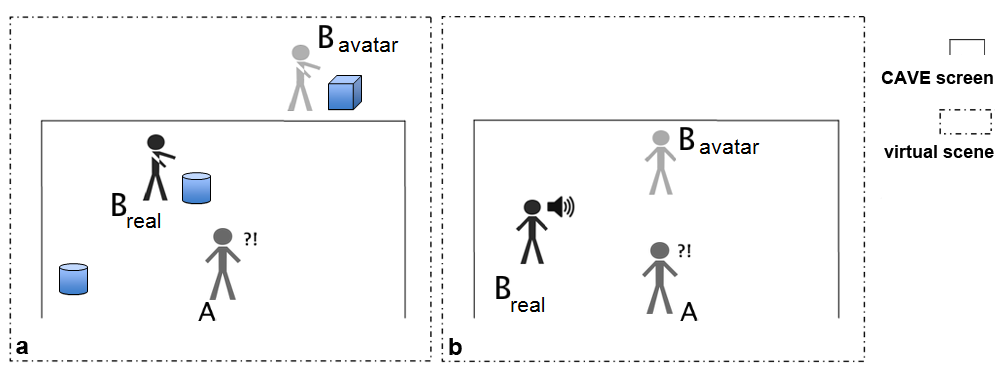
\includegraphics[width=\textwidth]{figures/ch2/inconsistency}
  \caption{\label{fig:2_inconsistency}Illustration of perceptual conflicts with a two-user scenario; user A interacts with avatar of user B: (a) Visual conflict occurs when user A simultaneously perceives the real user B and B's avatar pointing to different virtual objects. (b) Visual-audio conflict occurs when user B and the avatar are not at the same position.}
\end{figure}

\subsection{User Cohabitation}
Immersive virtual environment has the power to bring users to an artificial world by blocking the perception of the real world. In such situation users often forget boundaries of the physical workspace due to visual immersion, which could endanger both the user and the device. For some devices with non-closed display such as large image wall or a 3-wall CAVE, immersion is limited to the display area.

The human joystick metaphor does not necessarily prevent users from running into physical obstacles or keep user's field of view within projected areas. Moreover, if multiple users share the same immersive device for co-located collaboration with each one using a human joystick metaphor, they may have user cohabitation problems: users may run into collision when they move around without paying attention to other users (Figure~\ref{fig:2_illustration} left); one can also disrupt the visual perception of the virtual world of another if the former appears to be in the field of view of that user due to body occlusion (Figure~\ref{fig:2_illustration} right).

\begin{figure*}[tb]
  \centering
  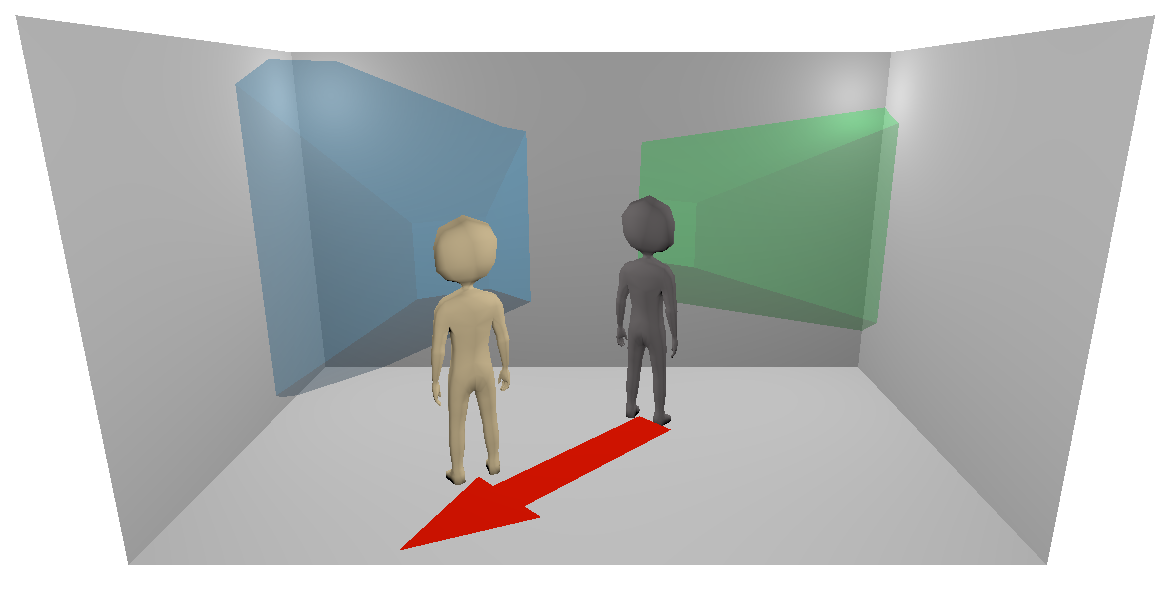
\includegraphics[width=0.49\textwidth]{figures/ch2/illu_col}
  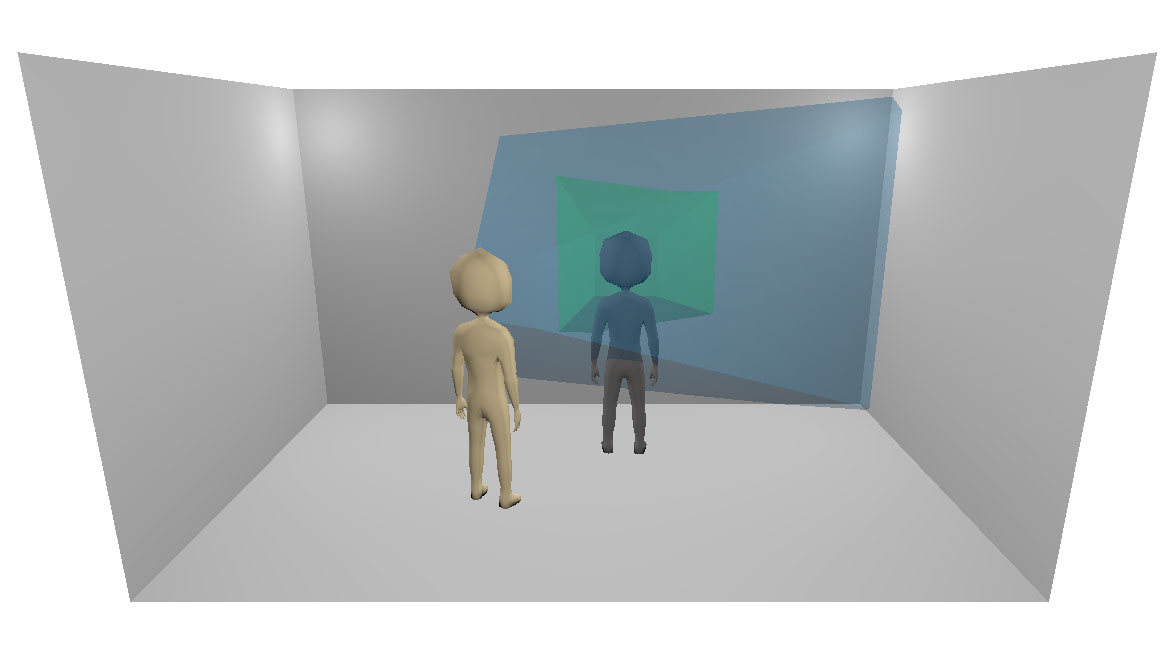
\includegraphics[width=0.49\textwidth]{figures/ch2/illu_occ}
  \caption{\label{fig:2_illustration}Illustration of collision (left) and occlusion (right) between co-located users in a multi-stereoscopic 3-wall plus floor CAVE.}
\end{figure*}

So to support safe and functional free navigation in an immersive context, the original human joystick metaphor should be adapted according to the number of co-located users and the configuration of the immersive system (size and shape of the screen walls, effective tracking space, etc.).

Two aspects of the problem should be solved: how to manage the spatial relationship between active users and the immersive display boundaries, i.e. how to prevent users from touching the wall screens and from seeing non projected areas, and how to provide enough workspace for each co-located user and thus avoid collision and occlusion between them.

When it comes to managing multiple users in the same immersive virtual environment for co-located collaboration, most works focused only on closely coupled collaboration (e.g. co-manipulation). In this case, virtual navigation is either disabled or controlled by a leader and shared by other users \citep{Beck2013IGG, Kulik2011CSS}. To enable more complex collaborative scenarios including loosely coupled tasks which require individual navigation for co-located users, we should propose novel navigation models that comply with user cohabitation constrains.

Table~\ref{tab:multi-user} shows a list of multi-user immersive displays.

\begin{table}[htb]
\renewcommand{\arraystretch}{1.3}
\caption{A List of Multi-user Displays.}
\label{tab:multi-user}
\centering
\begin{tabular}{p{3cm} l l l l l l}
  \hline
  Type & User Tracking & Number of Users \\ 
  \hline
  Omni-directional Stereo & No need & Large group \\
  \hline
  Multi-viewer Rendering Algorithm & All users & Two users (could be more) \\
  \hline
  Multi-monoscopic Display & All users & Two users \\
  \hline
  Multi-stereoscopic Display & All users & Two to six users \\
  \hline
  Multiple HMDs & All users & Depending on the room size \\
  \hline
\end{tabular}
\end{table}


% -------------------------------------------------------------------------------------------------


\section{Approach}
\subsection{Experiment}
\subsection{Iterative Paradigm Design}

\section{Chapter Summary}
